\documentclass[a4paper]{article}
\usepackage[utf8]{inputenc}
\usepackage[spanish, es-tabla, es-noshorthands]{babel}
\usepackage[table,xcdraw]{xcolor}
\usepackage[a4paper, footnotesep = 1cm, width=20cm, top=2.5cm, height=25cm, textwidth=18cm, textheight=25cm]{geometry}
%\geometry{showframe}

\usepackage{tikz}
\usepackage{amsmath}
\usepackage{amsfonts}
\usepackage{amssymb}
\usepackage{float}
\usepackage{graphicx}
\usepackage{caption}
\usepackage{subcaption}
\usepackage{multicol}
\usepackage{multirow}
\setlength{\doublerulesep}{\arrayrulewidth}
\usepackage{booktabs}
\usepackage{mathrsfs,amsmath}
\usepackage{hyperref}
\hypersetup{
    colorlinks=true,
    linkcolor=blue,
    filecolor=magenta,      
    urlcolor=blue,
    citecolor=blue,    
}

\newcommand{\quotes}[1]{``#1''}
\usepackage{array}
\newcolumntype{C}[1]{>{\centering\let\newline\\\arraybackslash\hspace{0pt}}m{#1}}
\usepackage[american]{circuitikz}
\usetikzlibrary{calc}
\usepackage{fancyhdr}
\usepackage{units} 

\graphicspath{./Imagenes}

\pagestyle{fancy}
\fancyhf{}
\lhead{22.05 ASSD}
\rhead{Mechoulam, Lambertucci, Rodriguez, Londero}
\rfoot{Página \thepage}

\begin{document}

%%%%%%%%%%%%%%%%%%%%%%%%%
%		Caratula		%
%%%%%%%%%%%%%%%%%%%%%%%%%

\begin{titlepage}
\newcommand{\HRule}{\rule{\linewidth}{0.5mm}}
\center
\mbox{\textsc{\LARGE \bfseries {Instituto Tecnológico de Buenos Aires}}}\\[1.5cm]
\textsc{\Large 22.05 Análisis de Señales y Sistemas Digitales}\\[0.5cm]


\HRule \\[0.6cm]
{ \Huge \bfseries Trabajo práctico N$^{\circ}$2}\\[0.4cm] 
\HRule \\[1.5cm]


{\large

\emph{Grupo 3}\\
\vspace{3px}

\begin{tabular}{lr} 	
\textsc{Mechoulam}, Alan  &  58438\\
\textsc{Lambertucci}, Guido Enrique  & 58009 \\
\textsc{Rodriguez Turco}, Martín Sebastian  & 56629 \\
\textsc{Londero Bonaparte}, Tomás Guillermo  & 58150 \\
\end{tabular}

\vspace{20px}

\emph{Profesores}\\
Jacoby, Daniel Andres\\
Belaustegui Goitia, Carlos F.\\
Iribarren, Rodrigo Iñaki\\
\vspace{3px}
%\textsc{} \\	

\vspace{100px}

\begin{tabular}{ll}

Presentado: & 15/05/20\\

\end{tabular}

}

\vfill

\end{titlepage}


%%%%%%%%%%%%%%%%%%%%%
%		Indice		%
%%%%%%%%%%%%%%%%%%%%%

%\tableofcontents
%\newpage

%%%%%%%%%%%%%%%%%%%%%
%		Informe		%
%%%%%%%%%%%%%%%%%%%%%

%\begin{center}
%	\Large{\textcolor{red}{\textbf{EN ROJO PONGO LO QUE HAY QUE HACER. NO BORRARLO HASTA NO TERMINARLO. RESPETAR FORMATOS.}} \textcolor{orange}{EN AZUL IDEAS DE QUE DESARROLLAR.}}
%\end{center}

\textbf{\textit{En el siguiente trabajo se presenta el estudio, investigación y análisis de un proceso de seguimiento del movimiento de un objeto en tiempo real, siendo conocida su posición inicial. Se realizaron pruebas tanto con videos como con cámaras web, pudiendo alternar el modo de trabajo.}}

%\textcolor{red}{\textbf{\textit{Resumen: falta mencionar ensayos y resultados.}}}

\section{Introducción}
Una imagen puede ser interpretada como una función bidimensional $f\left( x, y\right)$, donde tanto $x$ como $y$ representan en un plano el espacio visualizado, mientras que la misma función $f\left( x, y\right)$ es la intensidad de la imagen bajo un punto dado. Cuando $x$, $y$ y $f\left( x, y\right)$ son valores cuantizados y discretizados, la imagen se transforma en una imagen digital.

%f(x, y) como un campo vectorial cuya salida es un vector de intensidad y frecuencia
	 	
El procesamiento de dichas se define como el conjunto de técnicas aplicadas a estas imágenes, con el objetivo extraer información de ellas. Estas actividades cubren un campo que abarca un sin fin de aplicaciones, ya que se vale de maquinas capaces de detectar la totalidad del espectro electromagnético. Esto significa que se pueden obtener imágenes generadas por fuentes que captan información la cual para los humanos no se asocian con imágenes propiamente dichas, como lo son las ondas de radio, entre tantas otras.
	
Es posible considerar tres tipos de procesos computarizados en el procesamiento de imágenes, basándose en el nivel de tratamiento que se aplique, siendo así clasificados en bajo, medio y alto nivel. Los primeros incluyen actividades tales como reducción de ruido y aumento de contraste, tareas caracterizadas por el hecho de que tanto la entrada como la salida son imágenes. Las actividades de medio nivel de procesamiento incluyen trabajos de segmentación, es decir, identificar regiones u objetos dentro de las imágenes, descripción y clasificación de dichos elementos. Es así que esta categoría es destacada por sus salidas, ya que suelen ser información extraída de las imágenes a la entrada. Por último, los procesos de alto nivel se caracterizan por no solo reconocer objetos y analizarlos, sino también por darles un tratado normalmente asociado con la visión, tales así como ``darles sentido'' \cite{ref:intro1}.
	
%\textcolor{red}{Debe haber suficiente material para que un profesional que no conoce el tema para nada, pueda entenderlo. Referenciar libros y tutorial papers que profundicen.}
	
\section{Investigación}
Dada una señal continua a la entrada del sistema, una imagen sufre de dos procesos claves: \textbf{cuantización} y \textbf{discretización}. Si bien ambos refieren a tomar variables continuas y almacenarlas en memoria como variables discretas, se realiza esta diferenciación entre ambas ya que la primera hace referencia a la amplitud de la señal mientras que la segunda a coordenadas, que para el caso del estudio de imágenes, se refiere a pixeles, siendo estos el mínimo elemento que compone una imagen digital.
	
Ejemplificando lo anterior, se toma una entrada al sistema, como puede ser la presentada en la Figura (\ref{fig:disc1}), la cual, como ya se ha mencionado, es continua en $x$, $y$ y $f(x,y)$.
\begin{figure}[H]
\centering
	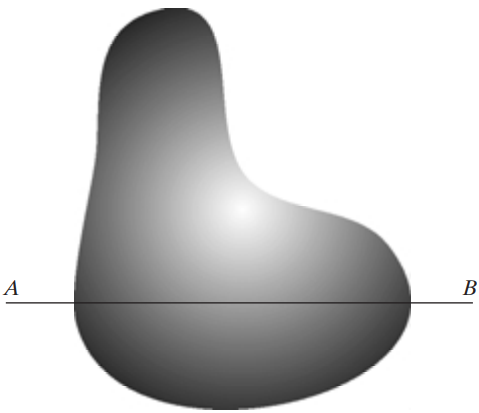
\includegraphics[width=0.3\textwidth]{Imagenes/Digitalizacion_1.png}
	\caption{Entrada continua al sistema.}
	\label{fig:disc1}
\end{figure}

Por lo tanto, se deben tomar coordenadas finitas, por ejemplo, aquellas que se encuentran sobre la recta AB, y asignarle a cada una un valor dado de amplitud. En la Figura~(\ref{fig:disc2}) se observa como una recta continua paralela al eje $x$ (horizontal), la cual posee ciertas variaciones aleatorias dadas por el ruido existente, es dividida en una cierta cantidad de posiciones equiespaciadas (discretización), marcadas con cuadrados blancos sobre la curva, asignándoles un nivel específico en la escala de grises (cuantización), marcado con una linea negra por la izquierda de dicha escala.
\begin{figure}[H]
\centering
	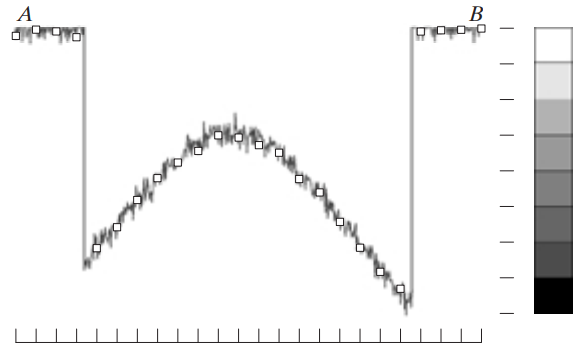
\includegraphics[width=0.4\textwidth]{Imagenes/Digitalizacion_2.png}
	\caption{Amplitud de la escala de grises en la recta AB y muestreo de valores.}
	\label{fig:disc2}
\end{figure}

Realizando el mismo proceso para todos los niveles de discretización en el eje $y$ (vertical), se obtiene finalmente una imagen digitalizada, la cual se la compara a continuación con la original \cite{ref:digit1}.
\begin{figure}[H]
\centering
	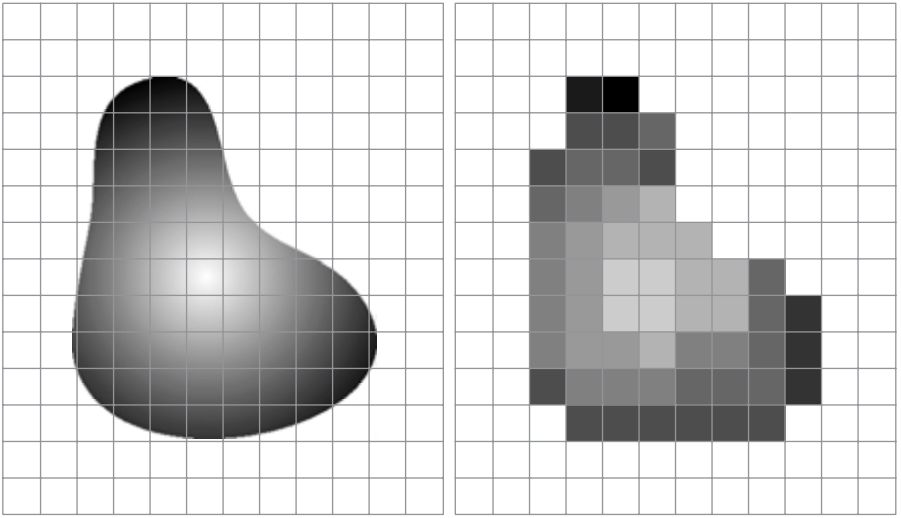
\includegraphics[width=0.5\textwidth]{Imagenes/Digitalizacion_3.png}
	\caption{Imagen original comparada con la imagen digitalizada a procesar.}
	\label{fig:disc3}
\end{figure}

\textcolor{red}{
\begin{itemize}
	%\item Descripción de las líneas de investigación (con referencias).
	\item Descripción de los conceptos más importantes de cada una.
	\item Análisis propio de lo presentado.
	\item Simulaciones de lo más relevante (códigos como apéndice).
	\item Elección del camino y justificación.
\end{itemize}
}
\textcolor{red}{Ehh... es necesario estos 4 puntos que quedaron? Yo pondría solo el código o algo así.}

Este trabajo se centra en procesos de medio nivel. Dicha definición es muy amplia, por lo cual es necesario acotar este camino. Es por ello que se decidió centrarse en el seguimiento de objetos en imágenes en movimiento. Se busco que, dada ciertas condiciones iniciales conocidas (brindadas por el usuario) en una imagen en movimiento en tiempo real, tomar un conjunto de datos de $x$, $y$ y $f(x,y)$ para así seleccionar un elemento y seguir su trayectoria a través del tiempo, como hipótesis plantearemos:
\begin{itemize}
\item El objeto no cambiará rápidamente de color ni su iluminación o exposición-
\item El objeto no sufrirá una oclusión por parte de un obstáculo del mismo color.
\end{itemize} para lograr este fin se utilizó el algoritmo de Lucas-Kanade de Optical Flow, el método de Shi-Tomasi, la utilización de filtros de Kalman y filtrado de color.
\subsection{Optical Flow} 
El campo de movimiento de una imagen es el movimiento real del objeto en el espacio proyectado sobre el plano de la imagen. El Optical Flow (flujo óptico) se define como el flujo de la intensidad en escala de grises en el plano de la imagen, a medida que evoluciona en el tiempo. También se puede interpretar el Optical Flow o flujo de la imagen como el movimiento aparente de la imagen  basado en la percepción visual, y tiene dimensión de velocidad $\vec{V}= (V_x \ , \ V_y)$. Si el Optical Flow se determina de dos imagenes consecutivas, aparece un vector de desplazamiento $\vec{d}$ de las cualidades elegidas, entre el cuadro n y el n+1.
\begin{figure}[H]
		\centering
		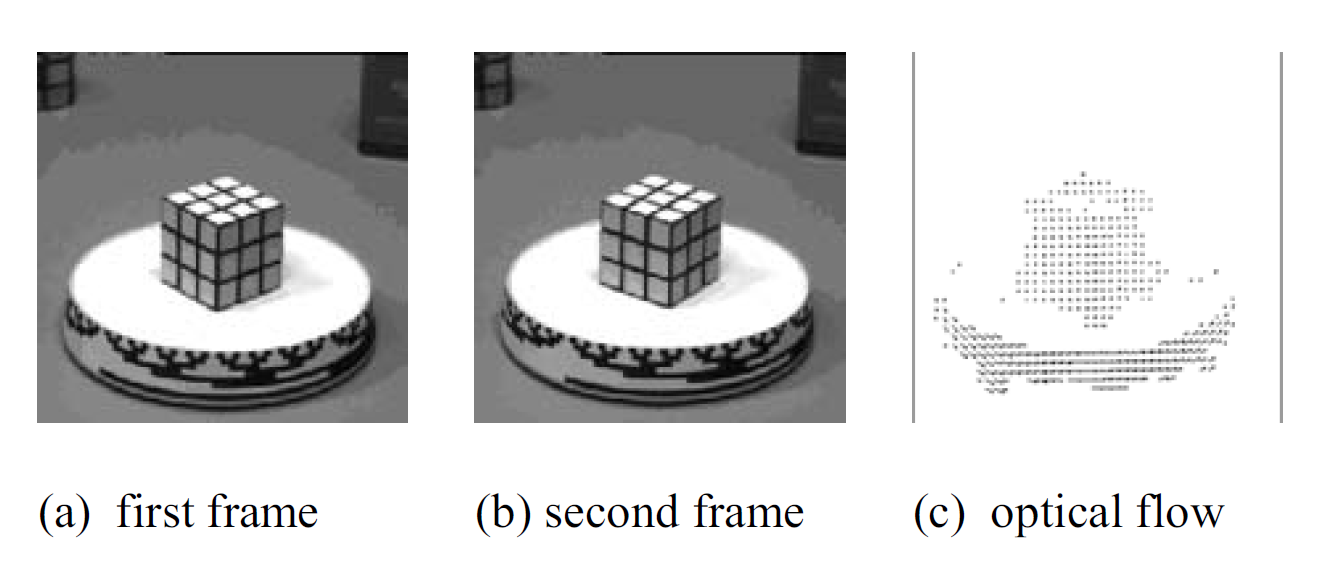
\includegraphics[width=0.5\textwidth]{Imagenes/opticalflowrubick.png}
		\caption{Cubo de rubik rotando en una mesa.}
		\label{fig:opticalflow1}
\end{figure}
Para la implementación del algoritmo existen varios caminos, como el basado en calculo de gradientes de la imagen total, existe otro que utiliza solo ciertos puntos que se determinan constantes de la imagen, nosotros utilizaremos el método piramidal de Lucas-Kanade.
\subsubsection{Lucas-Kanade} 
 Este consta del uso de información obtenida a partir de la intensidad del gradiente espacial para buscar la posición que mejor se acomoda a una imagen en movimiento \cite{ref:lucas-kanade} \cite{ref:lucas-kanade2}, algunas de las hipótesis que postula Lucas-Kanade son:
\begin{itemize}
\item Los movimientos entre cuadros consecutivos son pequeños. Tan pequeños como un pixel.
\item La intensidad de los objeto se mantiene constante cuadro a cuadro.
\end{itemize} 
Este algoritmo se basa en el principio de ``Divide y conquistarás'' al realizar la tarea de detectar movimiento en toda la imagen en problemas mas sencillos, consta de dividir la pantalla en un arbol cuaternario, y calculando recursivamente el optic flow de cada partición.
\begin{figure}[H]
		\centering
		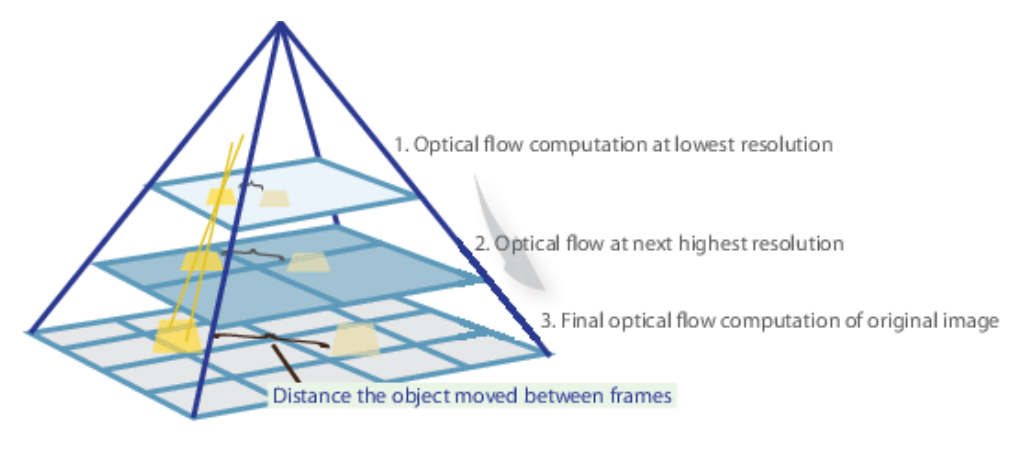
\includegraphics[width=0.5\textwidth]{Imagenes/op.png}
		\caption{Cálculo del Optical Flow.}
		\label{fig:opticalflow1}
\end{figure}

\subsection{Filtro de Kalman}

El filtro de Kalman es un filtro recursivo que busca estimar el estado de un sistema dinámico lineal discretizado de dimensión $n$ mediante una serie mediciones con ruido a partir de la descripción del modelo físico que rige las variables del vector de estado\cite{ref:kalman1}, \cite{ref:kalman2}.

\subsubsection{Planteo del problema}
Dado un proceso estocástico lineal en tiempo discreto definido por

\begin{equation}
x_k = Ax_{k-1} + w_{k-1} \footnote{Se omitió por simplicidad la función de control.}
\end{equation}

donde $x_k \in \mathcal{R}^{N}$ y siendo una medición en tiempo $k$ definida por

\begin{equation}
z_k = Hx_k + v_k
\end{equation}

con $z_k \in \mathcal{R}^m$, donde $w_k$ y $v_k$ son variables aleatorias que representan el ruido del proceso y de observación respectivamente, las cuales se asumen que son independientes entre sí y con distribuciones de probabilidad normales multivariadas definidas como

\[ p(w) \sim N(0, Q) \]

\[ p(v) \sim N(0, R) \]

donde $Q$ y $R$ son las matrices de covarianza del ruido del proceso y ruido de medición respectivamente, las cuales se asumen constantes; donde la matriz de transición de estados $A$ de dimensión $n\times n$ \textemdash siendo $n$ la dimensión de estados dinámicos del modelo\textemdash \ define la relación entre entados del paso $k-1$ al paso $k$ sin contar el ruido del proceso; donde la matriz de transición de observación $H$ de dimensión $m\times n$ \textemdash siendo $m$ la dimensión del vector de medición\textemdash \  fija la relación entre el espacio de  los observables medidos y el espacio de las variables del vector de estados, sin contar el ruido de medición; y finalmente donde el estado del filtro puede representarse como $\hat{x}_{k|k}$ y $P_{k|k}$, siendo estas el estimador del vector de estados a posteriori dadas las mediciones hasta un tiempo $k$, y el estimador de la matriz de covariaza a posteriori dadas las mediciones hasta un tiempo $k$ respectivamente. Se puede definir la operación del filtro de Kalman separando a esta en dos fases: la predicción, y la corrección.

\subsubsection{Ecuaciones de predicción}

\begin{equation}
\hat{x}_{k|k-1} = A\hat{x}_{k-1|k-1}
\end{equation}
\begin{equation}
P_{k|k-1} = AP_{k-1|k-1}A^T + Q
\end{equation}

\subsubsection{Ecuaciones de observación}

\begin{equation}
\hat{x}_{k|k} = \hat{x}_{k|k-1} + K_k y_k
\end{equation}
\begin{equation}
P_{k|k} = (\mathbb{I}-K_kH)P_{k|k-1}
\end{equation}

donde,

\begin{equation}
y_k = z_k - H\hat{x}_{k|k-1}
\end{equation}
\begin{equation}
S_k = HP_{k|k-1}H^T + R_k
\end{equation}
\begin{equation}
K_k = P_{k|k-1}H^TS_k^{-1}
\end{equation}

\begin{figure}[H]
		\centering
		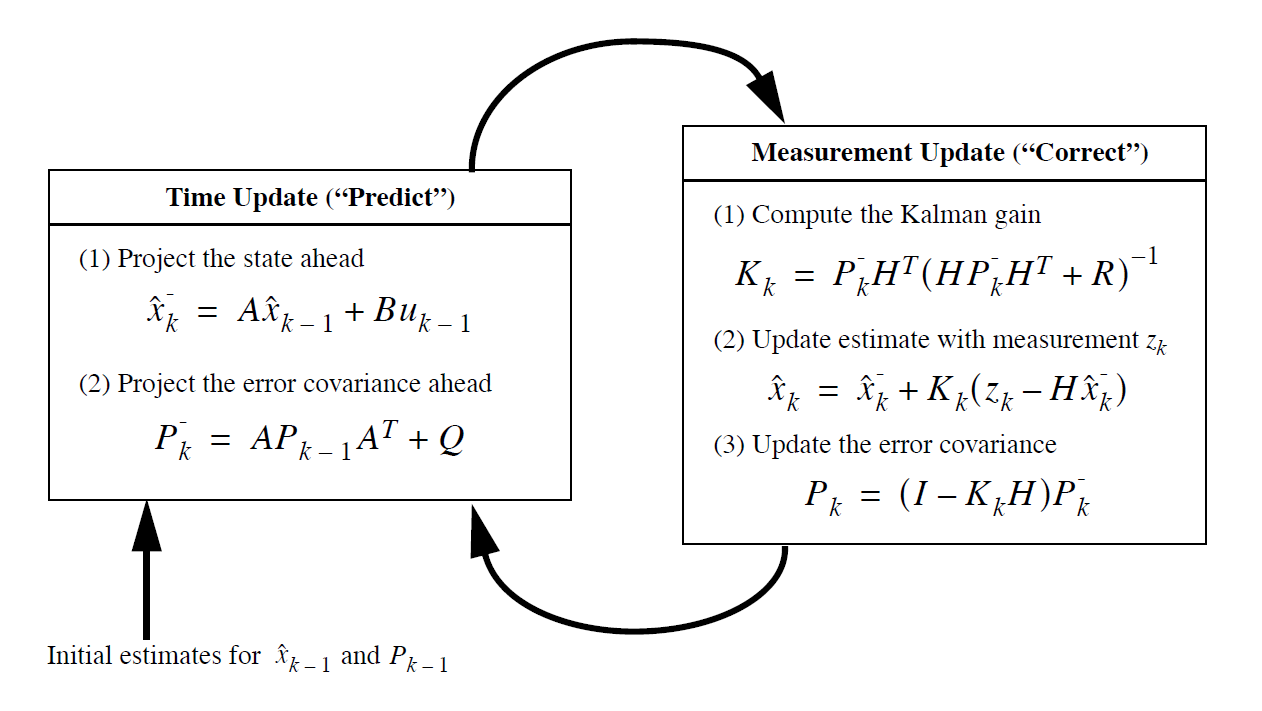
\includegraphics[width=0.5\textwidth]{Imagenes/kalman1.png}
		\caption{Funcionamiento completo del filtro Kalman simple \cite{ref:kalman2}.}
		\label{fig:kalman1}
\end{figure}

\subsubsection{Filtro de Color}
Se utilizó una máscara en todos los frames en base al color promedio de la selección inicial del usuario, el color promedio se obtiene al calcular la mediana de la selección.
 
\section{Aportes}

Se decidió implementar código en \textbf{Python}, apoyándose en la librería \href{https://opencv.org/}{OpenCV}.

Primero se desarrolló un programa capaz de realizar la estimación de una variable mediante el uso del filtro de Kalman. En la Figura (\ref{fig:kalman-comp}) se puede observar el funcionamiento del algoritmo con un vector de estados dinámicos de dimensión dos compuesto por las coordenadas $(x,y)$ sobre el plano cartesiano, realizando mediciones periódicamente. Se comparan dos curvas. Por un lado, una senoidal con un ruido gaussiano montado sobre ella, simulando una serie de mediciones con ruido, y por el otro lado, la estimación obtenida a partir del filtro desarrollado.

\begin{figure}[H]
\centering
	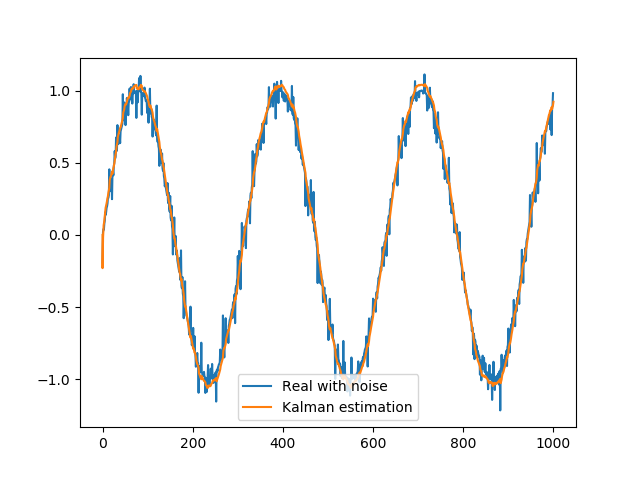
\includegraphics[width=0.4\textwidth]{Imagenes/Kalman_test_1.png}
	\caption{Seno con ruido comparada con estimación de Kalman.}
	\label{fig:kalman-comp}
\end{figure}


\subsection{Implementación}
A partir de una selección del video proporcionada por el usuario se obtienen las mejores features del objeto seleccionado utilizando el algoritmo de Shi-Tomasi. Luego, mediante el algoritmo de Lucas-Kanade de Optical Flow se obtiene la evolución de las features en el tiempo. A este cúmulo de puntos se le calcula el centro de masas $\mu$ y el centro de inercia $\sigma$. Se rechazan los puntos de este cúmulo que se encuentren a una distancia mayor a $k_{\sigma}\sigma$ respecto al centro de masas, para luego calcular nuevamente el centro de masas el cual es el que se introduce en el filtro de Kalman como medición de la posición.


Este algoritmo, hasta ahora explicado, cuenta con grandes problemas. Dados dos objetos $A$ y $B$, donde $A$ es el objeto a seguir:

\begin{itemize}
\item Como el algoritmo de Shi-Tomasi tiende a colocar features en bordes bien definidos, y estos suelen ser los bordes externos de un objeto, si el objeto a seguir $A$ pasa por delante de un objeto $B$ con bordes bien definidos, las features del algoritmo de Optical Flow tenderán a adosarse a los bordes del objeto $B$ por más que este esté quieto.
\item Si el objeto $A$ pasase por detrás del objeto $B$ inmóvil, todas las features sobre el objeto a seguir quedarían adosadas al objeto $B$. Esto plantea un problema mucho más grande que el anterior, dado que no se podrá utilizar la estimación del filtro de Kalman de manera confiable, debido a que cuando los features se queden quietos adosados en $B$, se seguirá midiendo de todas formas y se seguirán entregando esas mediciones al filtro de Kalman, por lo que la estimación de este se adosará también al objeto $B$.
\item Profundizando en el item anterior, existe una ambigüedad entre que $A$ pase de un movimiento MRU a que se quede completamente quieto y que $A$ pase por detras de $B$, dado que en ambas situaciones las features quedarán quietas en el lugar donde $A$ se haya quedado quieto o el lugar de la intersección entre $A$ y $B$
\end{itemize}

La mejora propuesta para sortear este problema consiste en agregar un filtro de color, para diferenciar a $A$ y a $B$ por su color. La implementación de este filtro de color comienza en el momento que el usuario selecciona el área a seguir. Se calcula la mediana del color de la zona elegida, y ese color es transformado de formato RGB a formato HSV, o Hue-Saturation-Value, dado que es más sencillo definir una máscara de este modo. Dado $x$ e $y$ las coordenadas de los píxeles de la imagen, $\vec{R_k}$, $\vec{G_k}$ y $\vec{B_k}$ los vectores de píxeles de la selección, $mediana(\vec{R_k}, \vec{G_k}, \vec{B_k}) = (m_R, m_G, m_B)$ el vector que define la mediana del color de la selección, $\mathbb{HSV}$ el operador de transformación del espacio de coordenadas RGB a HSV, y $\mathbb{HSV}(m_R, m_G, m_B) = (m_H, m_S, m_V)$ el vector de la mediana del color de la selección en el espacio HSV, queda entonces definida la máscara de color como

\begin{equation}
f(x, y) = (f_h(x, y), f_s(x, y), f_v(x, y))
\end{equation}

\begin{equation}
f_{u}(x,y) = \left\{
\begin{array}{ll}


      1 & -\Lambda_u < u_{x, y} - m_u < \Lambda_u \\
      
      
      
      0 & \text{sino} \\
      
      
\end{array} 
\right.
\end{equation}

donde $\Lambda$ es el límite para cada propiedad $u$, siendo estas Hue, Saturation o Value. Una vez obtenida la máscara $f(x, y)$ se realiza una operación AND bit-a-bit entre la máscara y la imagen original, logrando obtener una intensidad nula en los píxeles de la imagen que no posean un color cercano a la mediana calculada como se puede ver en las Figuras (\ref{fig:col1}) y (\ref{fig:col2}).

\begin{figure}[H]
\centering
	\begin{subfigure}{.4\textwidth}
		\centering
		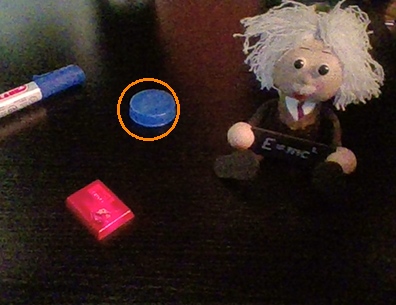
\includegraphics[width=\textwidth]{Imagenes/color1.png}
		\caption{Video antes de aplicar la máscara siguiendo al objeto azul.}
		\label{fig:col1}
	\end{subfigure}
	\begin{subfigure}{.4\textwidth}
		\centering
		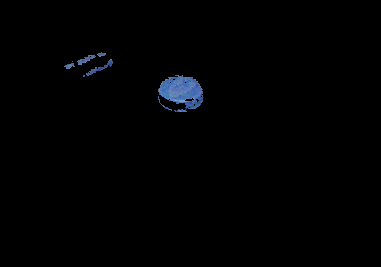
\includegraphics[width=\textwidth]{Imagenes/color2.png}
		\caption{Video después de aplicar la máscara. Es con esta imagen que opera el algoritmo y no con la normal.}
		\label{fig:col2}
	\end{subfigure}
	\caption{Comparación entre video normal y luego de aplicar la máscara.}
	\label{fig:color_comp}
\end{figure}

Este filtrado de color no solo posee una gran sinergia con el método de obtención de features de Shi-Tomasi, dado que este frame tendrá bordes de mucha mejor calidad, sino que tambíen posee una gran sinergia con el método de Optical Flow, debido a que como se verán menos bordes en la imagen modificada, aumenta notablemente la probabilidad de que los features queden contenidos todos dentro, o sobre los bordes del objeto a seguir.

Volviendo al caso de los objetos $A$ y $B$:

\begin{itemize}
\item Si $A$ y $B$ son de colores distintos, con el filtro de color el seguidor nunca detectará que existe un objeto $B$ por lo que seguirlo será imposible, y por consecuencia seguirá únicamente a $A$ y no se tendrá el problema de $A$ pasando por frente de $B$.
\item Si $A$ y $B$ son de colores distintos, y $A$, el objeto a seguir, pasa por detrás de $B$, ahora no se adosarán las features al objeto $B$, sino que el algoritmo verá que el área de $A$ se achica a medida que este queda oculto por $B$. Como los features no tendrán bordes para seguir, estos desaparecerán, por lo que se dejará de entregar mediciones al filtro de Kalman y este estimará correctamente la posición de $A$ mientras que este no haya sufrido aceleración alguna mientras estaba oculto. 
\end{itemize}

\begin{figure}[H]
\centering
	\begin{subfigure}{.4\textwidth}
		\centering
		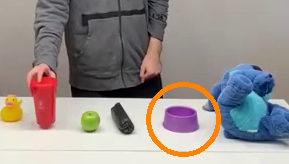
\includegraphics[width=\textwidth]{Imagenes/Optical1.png}
		\caption{Ventana con el funcionamiento normal del seguidor, el cual utiliza un círculo naranja para detallar donde se encuentra el objeto a seguir.}
		\label{fig:optical1}
	\end{subfigure}
	\begin{subfigure}{.4\textwidth}
		\centering
		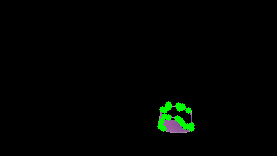
\includegraphics[width=\textwidth]{Imagenes/Optical2.png}
		\caption{Ventana la cual solo aparece al seleccionar el modo debug. Aquí se muestra si el filtro de color se encuentra activado, el video luego de pasar por la máscara de color, las features del objeto como puntos verdes y la zona de búsqueda si se diese el caso de tracking failure.}
		\label{fig:optical2}
	\end{subfigure}
	\caption{Resultado de la selección de un elemento.}
	\label{fig:optical12}
\end{figure}


\textcolor{red}{
\begin{itemize}
	\item Descripción y análisis de lo original producido por el grupo.
	\item Simulaciones que justifiquen las ideas, y que prueben su originalidad.
	\item Análisis de resultados
\end{itemize}
}

\section{Desarrollo}

\textcolor{red}{
\begin{itemize}
	\item Viabilidad, caminos alternativos.
	\item Proceso de implementación
	\item Documentación de los resultados: Resumen de lo más relevante, demos y programas van al apéndice.
	\item Evaluación y conclusiones del desarrollo.
\end{itemize}
}
\subsection{Posibles Mejoras}
Algunas mejoras que pueden ser implementadas en futuros desarrollos son:
\begin{itemize}
\item Trackeado multiobjeto:
Da la opción al usuario de trackear mas de un objeto en la pantalla.
\item Filtro de Kalman donde la matriz de covarianza de medición no sea constante:
En el modelo utilizado actualmente la matriz de covarianza es constante, esto asume que la presición de  medición es fija. Esto último no suele ser verdad en la realidad, una mejora es la introducción de modificaciones en la matriz de covarianza de manera dinámica así el filtro proporcionaría mejores predicciones, un caso en el que esto es vital es en la desaparición del objeto a trackear dado que en ese momento lo único utilizado es la predicción de Kalman. 
\item Filtro de sensibilidad Multicolor:
Dado tres objetos $A$ ,$B$ y $C$, donde $A$ cuenta con 2 colores distintivos, siendo estos rojo y azul, $B$ un objeto rojo y $C$ uno azul, lo que propone este filtro es la capacidad de diferenciar al objeto por mas de un color distintivo, cosa de que la interferencia de $B$ o $C$ en el camino de $A$ no comprometa su seguimiento.
\item Un mejor modelado de las ecuaciones dinámicas del filtro de Kalman para incluir la aceleración como variable de estado:
El modelo utilizado actualmente consta de un movimiento rectilíneo uniforme bidimensional, la inclusión de la aceleración proporcionaría una mejor predicción.
\end{itemize}




\subsection{Conclusiones}
Se logró seguimiento de un objeto especificado por el usuario en base a cualidades distintivas del mismo, siendo estas su color y su bordes, contando con una predicción certera en el caso de que se encuentre el objeto en pantalla al igual que la situación de que desaparezca de pantalla, aunque la varianza de la predicción aumentará cuanto mas tiempo no sea detectado el objeto, con la capacidad encontrar nuevamente el objeto.\\
La elección de los algoritmos y filtros utilizados son sinérgicos dado que estos se complementan entre sí, por ejemplo el filtro de color proporciona bordes definidos para el objeto a seguir, que es ideal para la obtención de bordes de Shi-Tomasi

\begin{thebibliography}{9}

\bibitem{ref:intro1}
R. C. Gonzalez, R. E. Woods y S. L. Eddins. \textit{Digital Image Processing Using MATLAB}. Prentice Hall, 2da ed, 2002.%, pp. 2-3.

\bibitem{ref:digit1}
R. C. Gonzalez, R. E. Woods y S. L. Eddins. \textit{Digital Image Processing Using MATLAB}. Prentice Hall, 2da ed, 2002, pp. 52-54.

\bibitem{ref:optic-flow}
D. H. Warren y Edward R. Strelow. \textit{Electronic Spatial Sensing for the Blind: Contributions from Perception}. Springer Netherlands, 1er ed, 1985. pp. 414.

\bibitem{ref:lucas-kanade}
B. D. Lucas y T. Kanade. \textit{An iterative image registration technique with an application to stereo vision}. De Proceedings of Imaging Understanding Workshop, pp. 121-130.

%\bibitem{ref:shi-tomasi}
%J. Shi y C. Tomasi. \textit{Good Features to Track}. 9th IEEE Conference on Computer Vision and Pattern Recognition, June 1994, Springer, pp. 593–600.

\bibitem{ref:lucas-kanade2}
W.S.P. Fernando, L. Udawatta , P. Pathirana. \textit{Identification of Moving Obstacles with Pyramidal
Lucas Kanade Optical Flow and k means
Clustering}. Faculty of Engineering, University of Moratuwa, Sri Lanka.

\bibitem{ref:kalman1}
G. Terejanu, "Discrete Kalman Filter Tutorial", Cse.sc.edu, 2020. [Online]. Available: https://cse.sc.edu/~terejanu/files/tutorialKF.pdf. [Accessed: 15- Jun- 2020].

\bibitem{ref:kalman2}
G. Welch and G. Bishop, An Introduction to the Kalman Filter. University of North Carolina at Chapel Hill: Department of Computer Science, 2006.

\end{thebibliography}

\end{document}